\section{lemma5}
\begin{lemma}
\end{lemma}
Suppose we have a Riemann sphere $C$ and a diagram $(C,\iota,\xi)$ and a regular cell complex refinement $\overline{(C,\iota,\xi)}$ and a sheaf $\mathfrak{F}$ singular supported on it such that when restricted to a small disk $D\subset C$ the refinement is as the following figure :

\begin{figure}[H] % Optional: [h] means here, [t] for top, [b] for bottom, [p] for page of floats
    \centering
    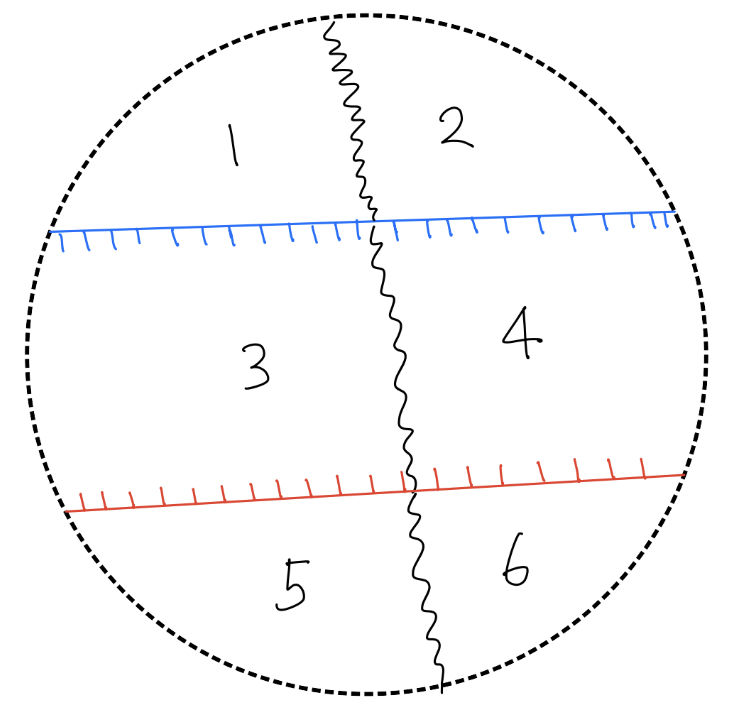
\includegraphics[width=\linewidth]{diagrams/lemma5/1.png} % Adjust the width as needed
    \caption{Your caption here}
    \label{fig:your-label}
\end{figure}

Stalks :\\

- 1 : $\mathbb{C}^{m+1}$\\
- 2 : $\mathbb{C}^{m+1}$\\
- 3 : $\mathbb{C}^{m}$\\
- 4 : $\mathbb{C}^{m}$\\
- 5 : $\mathbb{C}^{m+1}$\\
- 6 : $\mathbb{C}^{m+1}$\\


Let $T$ be a block diagonal matrix of size $(1,m,1)$. We denote the submatrix of $T$ with index range $a\leq i \leq b$,$a\leq j \leq b$ to be $T_{a,b}$. \\

Let m be arbitrary positive integer, then we denote the inclusion map from $\mathbb{C}^{m}$ to $\mathbb{C}^{m+1}$ that sends $e_i$ to $e_i$($e_{i+1}$ resp.) by $\iota_f$($\iota_l$ resp.)\\

Generization maps :\\

- 1$\rightarrow$2 : $T_{1,m+1}$\\
- 3$\rightarrow$4 : $T_{2,m+1}$\\
- 5$\rightarrow$6 : $T_{2,m+1}$\\
- 3$\rightarrow$1 : $\iota_l$\\
- 4$\rightarrow$2 : $\iota_l$\\
- 3$\rightarrow$5 : $\iota_f$\\
- 4$\rightarrow$6 : $\iota_f$\\

Now we apply a sequence of isotopies to $\mathfrak{F}$ which will be called $isotopy_5$ :\\

(step1) Inside the disk surrounded by purple circle apply $isotopy_1$

\begin{figure}[H] % Optional: [h] means here, [t] for top, [b] for bottom, [p] for page of floats
    \centering
    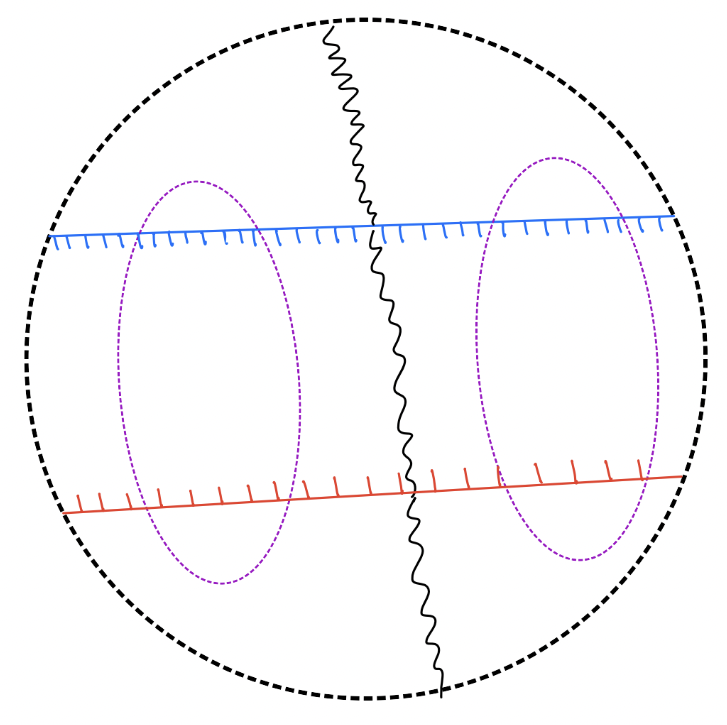
\includegraphics[width=\linewidth]{diagrams/lemma5/2.png} % Adjust the width as needed
    \caption{Your caption here}
    \label{fig:your-label}
\end{figure}

we get the following diagram :
\begin{figure}[H] % Optional: [h] means here, [t] for top, [b] for bottom, [p] for page of floats
    \centering
    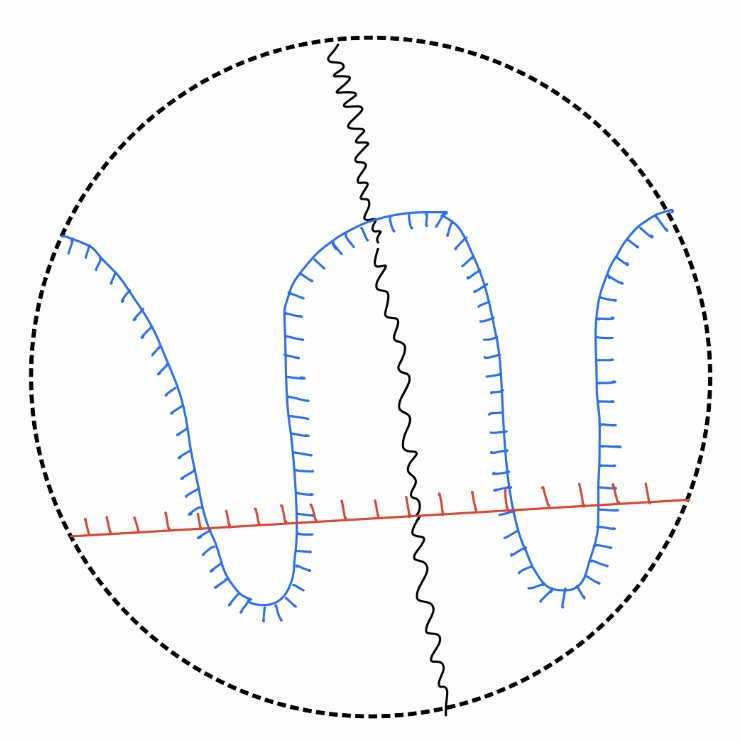
\includegraphics[width=\linewidth]{diagrams/lemma5/3.png} % Adjust the width as needed
    \caption{Your caption here}
    \label{fig:your-label}
\end{figure}
(step2) Now apply $isotopy_3$ inside the disk surrounded by the purple circle:
\begin{figure}[H] % Optional: [h] means here, [t] for top, [b] for bottom, [p] for page of floats
    \centering
    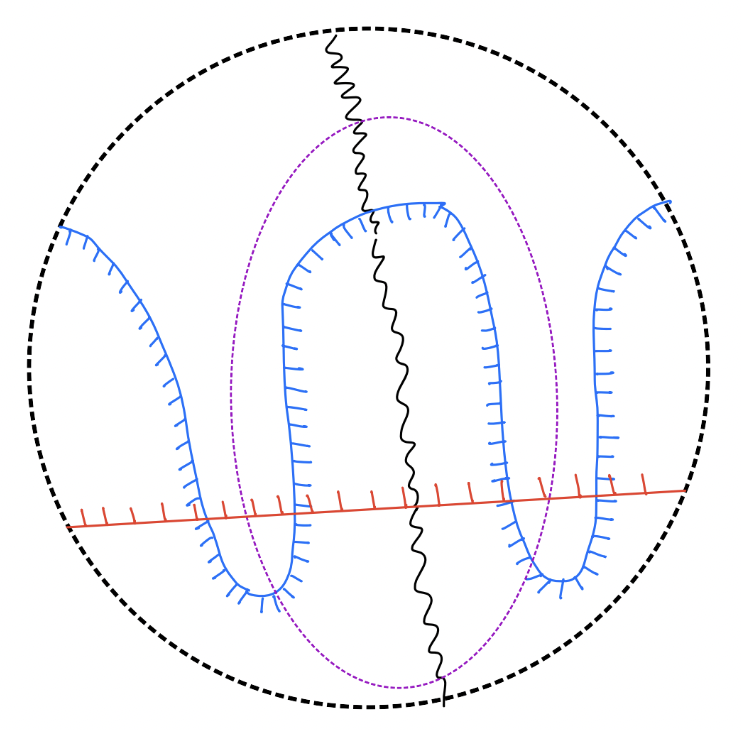
\includegraphics[width=\linewidth]{diagrams/lemma5/4.png} % Adjust the width as needed
    \caption{Your caption here}
    \label{fig:your-label}
\end{figure}

We get the following diagram and a sheaf :

\begin{figure}[H] % Optional: [h] means here, [t] for top, [b] for bottom, [p] for page of floats
    \centering
    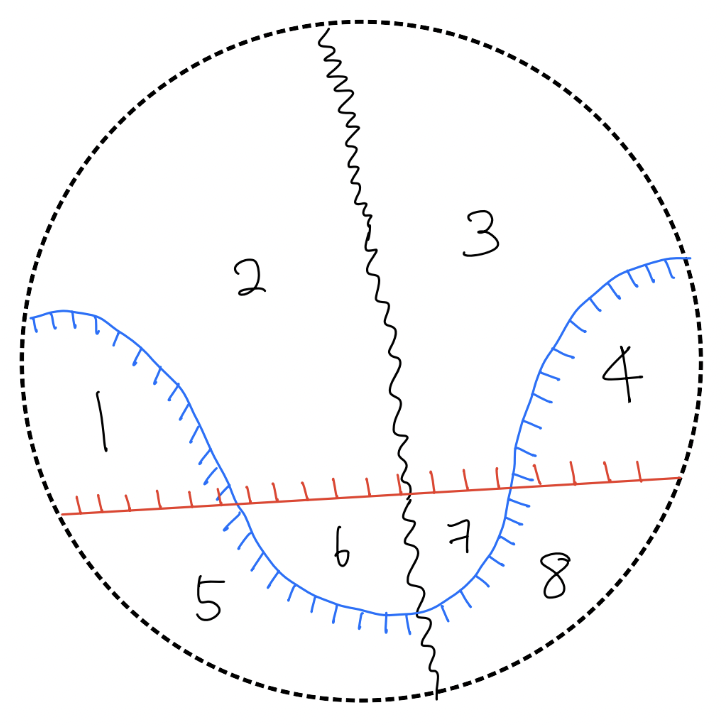
\includegraphics[width=\linewidth]{diagrams/lemma5/5.png} % Adjust the width as needed
    \caption{Your caption here}
    \label{fig:your-label}
\end{figure}

Stalks : \\
- 1 : $\mathbb{C}^{m}$\\
- 2 : $\mathbb{C}^{m+1}$\\
- 3 : $\mathbb{C}^{m+1}$\\
- 4 : $\mathbb{C}^{m}$\\
- 5 : $\mathbb{C}^{m+1}$\\
- 6 : $\mathbb{C}^{m+2}$\\
- 7 : $\mathbb{C}^{m+2}$\\
- 8 : $\mathbb{C}^{m+1}$\\

Generization maps : \\


- 1$\rightarrow$2 : $\iota_l$\\
- 4$\rightarrow$3 : $\iota_l$\\
- 1$\rightarrow$5 : $\iota_f$\\
- 4$\rightarrow$8 : $\iota_f$\\
- 2$\rightarrow$6 : $\iota_f$\\
- 3$\rightarrow$7 : $\iota_f$\\
- 5$\rightarrow$6 : $\iota_l$\\
- 8$\rightarrow$7 : $\iota_l$\\
- 2$\rightarrow$3 : $T_{1,m+1}$\\
- 6$\rightarrow$7 : $T_{1,m+2}$\\
- 5$\rightarrow$8 : $T_{2,m+2}$\\

(proof) After (step1), by lemma1, we get the following sheaf :
\begin{figure}[H] % Optional: [h] means here, [t] for top, [b] for bottom, [p] for page of floats
    \centering
    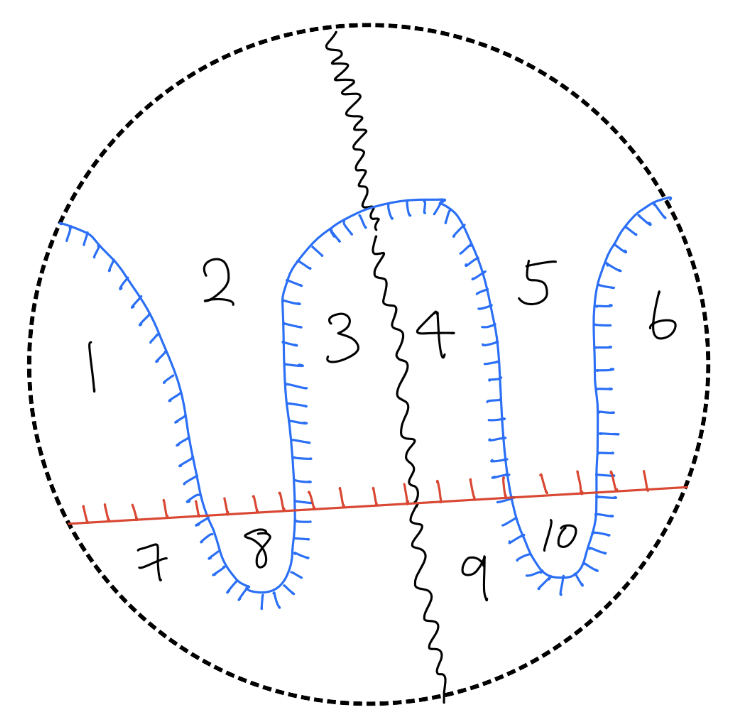
\includegraphics[width=\linewidth]{diagrams/lemma5/6.png} % Adjust the width as needed
    \caption{Your caption here}
    \label{fig:your-label}
\end{figure}

Stalks : \\
- 1 : $\mathbb{C}^{m}$\\
- 2 : $\mathbb{C}^{m+1}$\\
- 3 : $\mathbb{C}^{m}$\\
- 4 : $\mathbb{C}^{m}$\\
- 5 : $\mathbb{C}^{m+1}$\\
- 6 : $\mathbb{C}^{m}$\\
- 7 : $\mathbb{C}^{m+1}$\\
- 8 : $\mathbb{C}^{m+2}$\\
- 9 : $\mathbb{C}^{m+1}$\\
- 10 : $\mathbb{C}^{m+2}$\\

Generization maps : \\


- 1$\rightarrow$2 : $\iota_l$\\
- 3$\rightarrow$2 : $\iota_l$\\
- 4$\rightarrow$5 : $\iota_l$\\
- 6$\rightarrow$5 : $\iota_l$\\
- 1$\rightarrow$7 : $\iota_f$\\
- 3$\rightarrow$7 : $\iota_f$\\
- 4$\rightarrow$9 : $\iota_f$\\
- 6$\rightarrow$9 : $\iota_f$\\
- 2$\rightarrow$8 : $\iota_f$\\
- 7$\rightarrow$8 : $\iota_f$\\
- 5$\rightarrow$10 : $\iota_f$\\
- 9$\rightarrow$10 : $\iota_l$\\
- 2$\rightarrow$5 : $T_{1,m+1}$\\
- 3$\rightarrow$4 : $T_{2,m+1}$\\
- 7$\rightarrow$9 : $T_{2,m+2}$\\

Now to the above sheaf we apply (step2), then by lemma3, we get the final sheaf.